\documentclass{standalone}

\usepackage{tikz}
\begin{document}
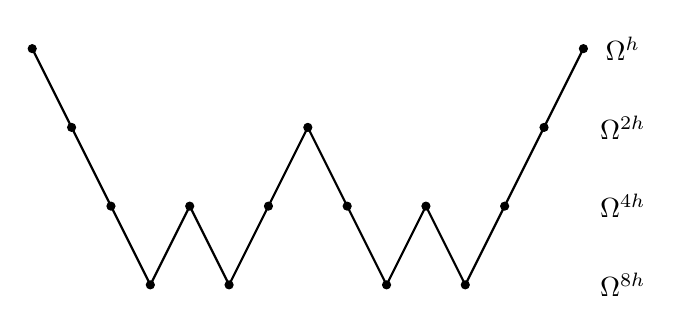
\begin{tikzpicture}
  \filldraw (0, 2) circle (0.02in);
  \filldraw (-0.5, 1) circle (0.02in);
  \filldraw (0.5, 1) circle (0.02in);
  \filldraw (-1, 0) circle (0.02in);
  \filldraw (1, 0) circle (0.02in);
  \filldraw (-1.5, 1) circle (0.02in);
  \filldraw (1.5, 1) circle (0.02in);
  \filldraw (-2, 0) circle (0.02in);
  \filldraw (2, 0) circle (0.02in);
  \filldraw (-2.5, 1) circle (0.02in);
  \filldraw (2.5, 1) circle (0.02in);
  \filldraw (-3, 2) circle (0.02in);
  \filldraw (3, 2) circle (0.02in);
  \filldraw (-3.5, 3) circle (0.02in);
  \filldraw (3.5, 3) circle (0.02in);
  \draw[thick] (0, 2) -- (-1,0);
  \draw[thick] (0, 2) -- (1,0);
  \draw[thick] (-1, 0) -- (-1.5,1);
  \draw[thick] (1, 0) -- (1.5,1);
  \draw[thick] (-1.5, 1) -- (-2,0);
  \draw[thick] (1.5, 1) -- (2,0);
  \draw[thick] (-2, 0) -- (-3.5,3);
  \draw[thick] (2, 0) -- (3.5,3);
  \node at (4, 3)  {$\Omega^h$};
  \node at (4, 2)  {$\Omega^{2h}$};
  \node at (4, 1)  {$\Omega^{4h}$};
  \node at (4, 0)  {$\Omega^{8h}$};
\end{tikzpicture}
\end{document}